\documentclass[pdftex,12pt,letter]{article}
\usepackage[binary-units=true]{siunitx}
\usepackage[margin=0.75in]{geometry}
\usepackage[utf8]{inputenc}
\usepackage[T1]{fontenc}
\usepackage{graphicx}
\usepackage{amsmath}
\usepackage{xspace}
\usepackage{xcolor}
\usepackage[pdftex,pdfpagelabels,bookmarks,hyperindex,hyperfigures]{hyperref}

\newcommand{\fixme}[1]{\textcolor{red}{\textit{Fixme}: \textbf{#1}}}


\author{Brett Viren}
\date{\today \\ \textcolor{red}{(draft version 0.3)}}
\title{Single-Phase protoDUNE TPC Numbers}
\begin{document}

\maketitle

\begin{abstract}
  The numbers relevant to the Time Projection Chamber (TPC) data for
  the single-phase protoDUNE experiment is described.  They are given
  in terms of a hierarchy of the detector parts relevant to TPC data.
  A set of global or ``flat'' numbering is proposed.  \fixme{Note,
    while in draft, things are subject to change.}
\end{abstract}

%\newpage
\tableofcontents
\newpage
\section{Overview}

This document describes the numbers involved in labeling parts of the
single-phase protoDUNE detector related to the TPC.  A family of
labels are defined to refer to these detector parts in this note.
These labels can not possibly coincide with those used to describe the
part in every context. 

The document addresses the parts roughly in the order that information
flows starting from ionization activity in the liquid argon and ending
with raw data on disk.  For each part, the numbering convention used
by its producers is given.  In some cases, relevant numbering invented
by others is given for reference and to facilitate transforming sets
of numbers between the context presented in this note and others.

The rest of this overview gives a description of the detector part
hierarchy relevant to the numbering, an orientation of the detector
and a family of coordinate systems which are used to describe the
numbering.  Subsequent sections are devoted to the part numbering
themselves.  The note ends with a section proposing ways to flatten
the hierarchy of numbers in order to produce global numbering.

\subsection{Detector Parts}
\label{sec:parts}

For the purpose of this note, the single-phase protoDUNE detector is
considered to be composed of the following hierarchy of parts.  The
part list necessarily is not complete.  Rather, it focuses on the
parts that impact how data may be addressed.

\begin{description}
\item[Detector] is a logical boundary for that which contains TPCs.
\item[TPC] (aka ``drift cell'') is a volume of liquid argon bounded on one side by an Anode
  Plane Assembly (APA) face and the other either by a Cathode Plane
  Assembly (CPA) or by a detector wall.
\item[APA] consists of a metal frame on which wires and cold
  electronics are mounted.  It is logically split into two APA \textit{faces}.
\item[APA face] includes a number of active \textit{wire
    planes} (among other things).
\item[Wire plane] consists of a number of (nominally) parallel
  \textit{wires}, spanning the APA face.  In the direction of drift
  these planes are named here in alphabetical order: \textbf{U},
  \textbf{V} and \textbf{W}.  The first two are also termed
  ``induction'' planes and the last one
  ``collection''.\footnote{Despite the fact that all three collect
    induced signals.}
\item[Wire] or more correctly a
  \textit{wire segment} is one (nominally) straight run of a \textit{conductor}.
\item[Conductor] is one or more sensitive wire segments, possibly
  wrapping around an APA, which is ultimately attached to an input
  electronics channel.
\item[ASIC] is used generically here to mean either a front-end
  electronic (FEE) amplifier ASIC or its paired ADC ASIC.
\item[Channel] is associated with the amplification, digitization and
  readout of one conductor.
\item[Wire board] provide the physical and electrical termination for
  a set of segment-0 wires.
\item[CR board] boards holding resistors and capacitors through which
  the wires are electrically connected to the FEE ASIC input.
\item[FEMB] is the front-end motherboard holding a number of ASICs and
  with a number of wires.
\item[Cold FPGA] is responsible to multiplex the outputs from the ADCs
  on the FEMB to a WIB.
\item[WIB] is a warm-interface board which is associated with a
  number of FEMBs in an APA.
\item[Readout] is either an RCE or a FELIX device which is associated
  with a number of WIBs.
\item[DAQ] is the distributed computer application based on artDAQ
  which accepts data from readout devices, collates their fragments
  based on trigger information, and writes the result to file.
\end{description}



In this note \textit{local
  numbering} describes how one part in this hierarchy relates to its
parent and to sibling instances.  Local numbers may be duplicated as
parent (or grandparent, etc) parts are replicated across the detector.
As such an as-designed symmetry is assumed.  If any significant
as-built deviations occur they must be understood and documented.  The
system to handle these deviations is out of scope for this document.  

\subsection{Orientation}

The installation group defines a descriptive orientation labeling.  It
is defined in approximate alignment with the direction of the particle
beam from CERN.  It is reproduced in table~\ref{tab:global}.

\begin{table}[htp]
  \label{tab:global}
  \centering
  \begin{tabular}[h]{|c|c|c|}
    \hline
    \multicolumn{3}{|c|}{North, aka ``Beam-Left''} \\
    \hline
    Upstream & Midstream & Downstream \\
    \hline
    \multicolumn{3}{|c|}{South, aka ``Beam-Right''} \\
    \hline
    \multicolumn{3}{c}{$\longrightarrow$ approximate beam direction $\longrightarrow$} \\    
  \end{tabular}
  \caption{Global orientation labels from the installation group.
    Beam travels approximately left to right.  Up-, mid- and
    down-stream may be abbreviated US, MS and DS, respectively.
    Beam-left (BL) and beam-right (BR) are on the North and South
    sides of the detector, respectively.}
\end{table}

\subsection{Coordinate Systems}
\label{sec:coordsys}

A family of Cartesian coordinate systems is adopted in this note to
assist in describing the numbering.  Their coordinates are defined and
their semantic meanings are summarized as:

\begin{description}
\item[Global] $(x_g, y_g, z_g)$ is associated with
  some ``lab frame'' but need not be defined further here.
\item[Detector] $(x_d, y_d, z_d)$ is defined with respect to the
  \textit{global} system and has axes aligned with the detector such
  that $y_d$ points upward, counter to gravity, $z_d$ points
  transverse to the nominal drift direction and approximately in the
  direction of the beam and $x_d$ follows from the right-hand-rule and
  is either parallel or anti-parallel to the nominal (local) electron
  drift direction.  The origin of this coordinate system is left
  unspecified here.
\item[Chamber] $(x_c, y_c, z_c)$ is defined with respect to the
  \textit{detector} coordinate system.  There is one chamber
  coordinate system for each TPC.  For each chamber, the $y_c$
  direction is parallel to that of the \textit{detector} system, the
  $x_c$ direction is normal to the APA face associated with the
  chamber and $z_c$ follows from right-hand-rule.  The origin of both
  the $y_c$ and $z_c$ axes is chosen to be at the center of the active
  area of the APA face.  The $x_c$ origin lies on the center plane
  that divides the APA into two faces.
\item[Wire] $(x_w, y_w, z_w)$ is defined with respect to a
  \textit{chamber} coordinate system.  There is one wire coordinate
  system associated with each wire plane in the APA face bounding the
  chamber.  The $x_w$ axis is identified with $x_c$.  The $y_w$ axis
  points along the wire in the direction (positive) current flows
  toward the electronics.  The $z_w$ follows from the right-hand-rule
  and points in the direction of the \textit{wire pitch}.  The origin
  of the wire coordinate system is identified with that of the chamber
  system.  They are related by a rotation but not a
  translation.  Note, for W-planes, the wire and chamber coordinate
  systems are identical.
\end{description}

\noindent These last two categories of coordinate systems are illustrated in Figure~\ref{fig:coords}.

\begin{figure}[htp]
  \centering
  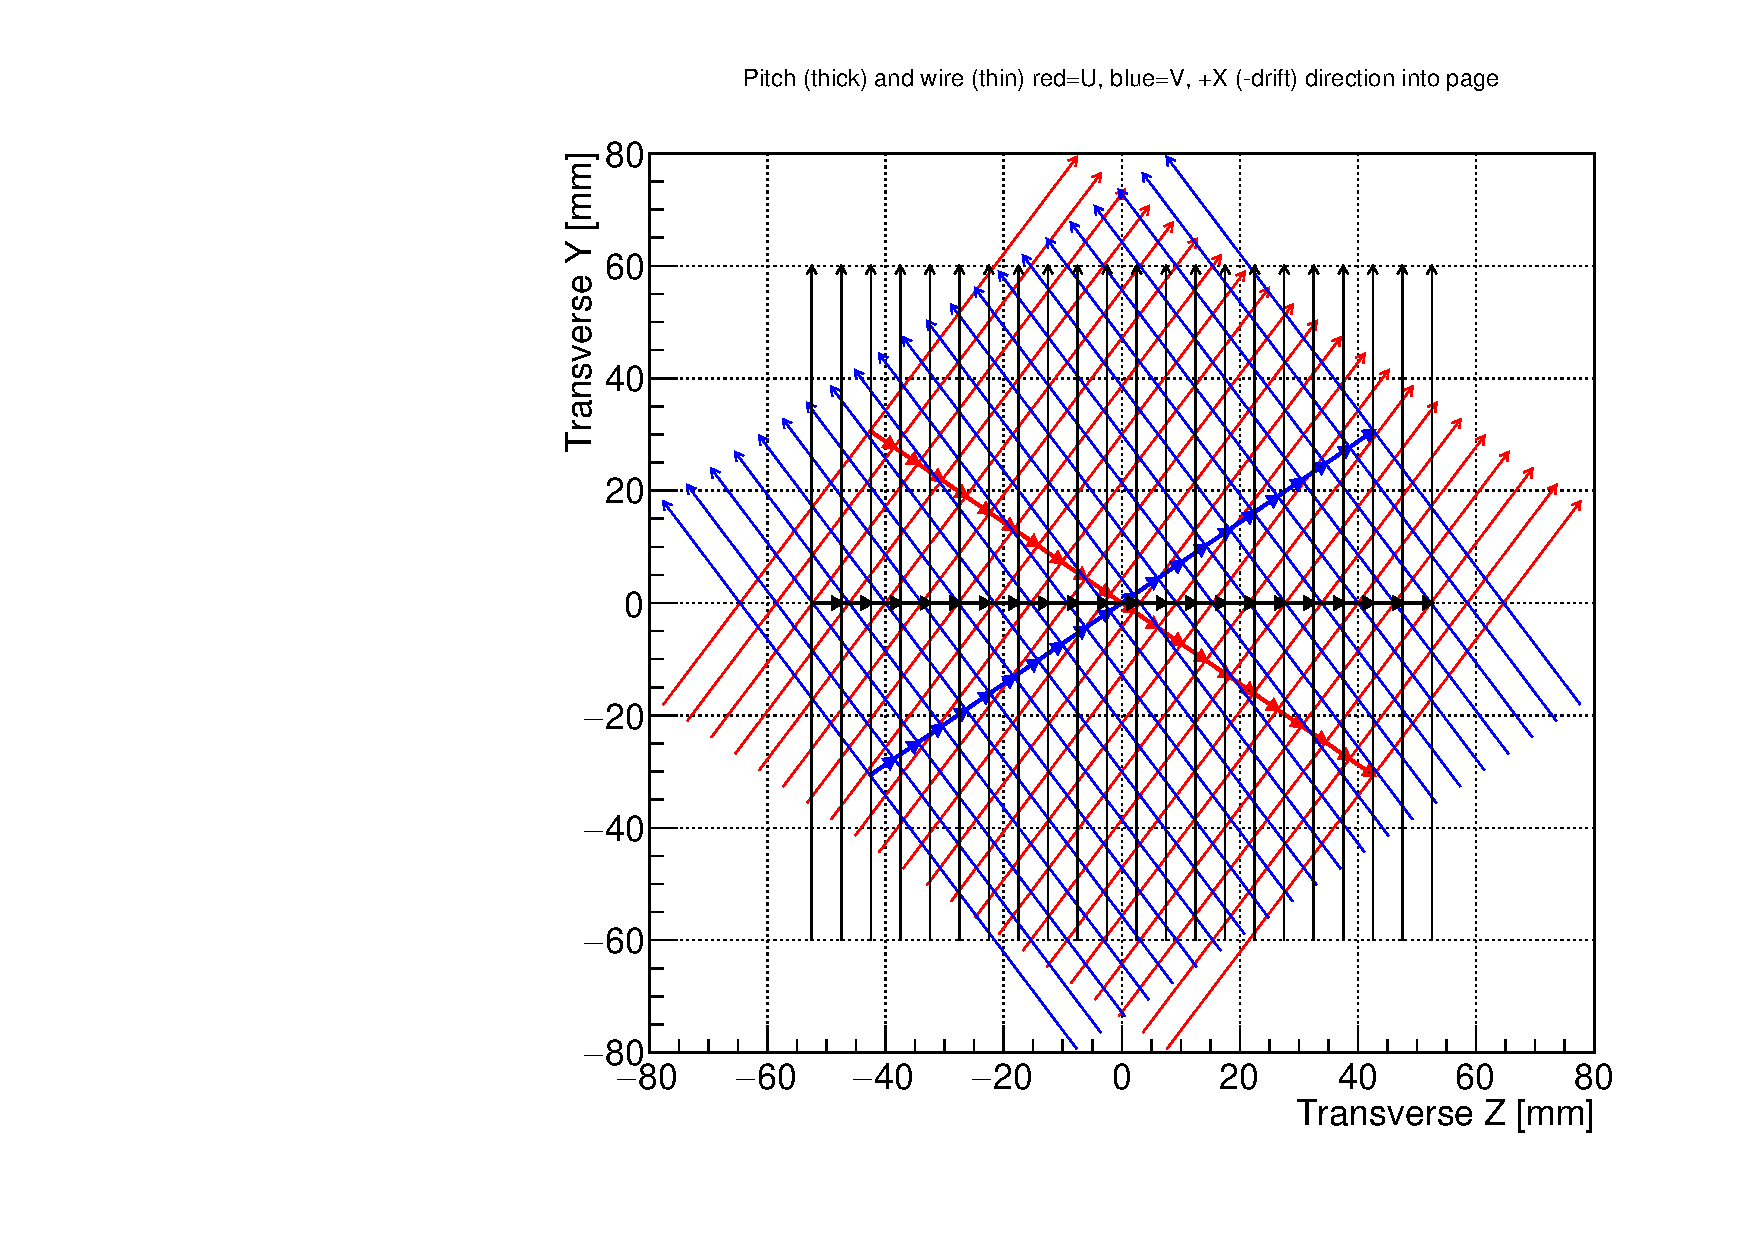
\includegraphics[width=0.8\textwidth]{test_pimpos_draw.pdf}
  \caption{Illustration of the three wire coordinate systems relative to their parent chamber coordinate system, limited to the transverse plane.  For each plane \textcolor{red}{U in red}, \textcolor{blue}{V in blue} and \textbf{W in black}, the thin arrows are along the wire ($y_w$) direction, the thick arrows are along the pitch ($z_w$) direction. The axes of the plot represent the $y_c$ and $z_c$ axes.  Into the page are the common $x_c$ and the three $x_w$ for each plane.  Note: these coordinate systems are used to describe the numbering in this note and may not be in use in every context.}
  \label{fig:coords}
\end{figure}


\section{Chambers}

The detector is composed of two types of logical chambers (aka TPC
drift cells).  There are 6 ``inner'', ``large'' or ``central''
chambers that are bounded by an APA face and a CPA.  The face on the
opposite side of their APA bounds a ``outer'', ``thin'' or ``edge''
chamber which is further bounded by a detector wall.  The
electrostatic field in this chamber is such that most ionized
electrons produced therein are not detected.

The raw data contains no chamber numbers, per se.  However, the data
must identify FEMBs one APA face or the other and faces are one-to-one
correlated to chambers.  The important inner chamber numbers used here
follow the APA numbers given below.  The outer chamber numbers follow
with each one six higher than the chamber on the inner face of the
shared APA and are listed in table~\ref{tabl:tpc}.

It's worth contrasting these numbers with the current LArSoft TPC
numbering which rasters a count in ``drift-major'' order and
irrespective of the difference between edge and central TPCs.  See
table~\ref{tab:lstpc} for a corresponding description.

\begin{table}[htp]
\begin{minipage}{0.4\textwidth}
  \centering
  \begin{tabular}[h]{|c|c|c|}
    \hline\hline
    12 & 11 & 10\\
    \hline
    \hline
    \multicolumn{3}{|c|}{APAs}\\
    \hline
    \hline
    6 & 5 & 4 \\
    \hline
    \hline
    \multicolumn{3}{|c|}{CPAs}\\
    \hline
    \hline
    3 & 2 & 1 \\
    \hline
    \hline
    \multicolumn{3}{|c|}{APAs}\\
    \hline
    \hline
    9 & 8 & 7 \\
    \hline
    \hline
    \multicolumn{3}{c}{beam $\longrightarrow$} \\    
  \end{tabular}
  \caption{The \textbf{chamber} (TPC drift cell) numbering which
    follows the APA numbering used by the installation group.}
  \label{tab:tpc}
\end{minipage}\hfill
\begin{minipage}{0.4\textwidth}
  \centering
  \begin{tabular}[h]{|c|c|c|}
    \hline\hline
    3 & 7 & 11\\
    \hline
    \hline
    \multicolumn{3}{|c|}{APAs}\\
    \hline
    \hline
    2 & 6 & 10 \\
    \hline
    \hline
    \multicolumn{3}{|c|}{CPAs}\\
    \hline
    \hline
    1 & 5 & 9 \\
    \hline
    \hline
    \multicolumn{3}{|c|}{APAs}\\
    \hline
    \hline
    0 & 4 & 8 \\
    \hline
    \hline
    \multicolumn{3}{c}{beam $\longrightarrow$} \\    
  \end{tabular}
  \caption{Current LArSoft TPC numbering taken from dunetpc wiki~\cite{dunetpc-wiki}.  These are not proposed for convention. \fixme{Check is beam direction/number correlation is correct.}}
  \label{tab:lstpc}
\end{minipage}\hfill
\end{table}


\section{APA}

Each APA is an independent data source for the artDAQ based DAQ.  It
is the ``Board Reader'' node of the DAQ which assigns APA
number.\fixme{Right?}  The APA numbering of the installation group is
described in table~\ref{tab:apa}.  As stated above, an inner chamber
number matches the number of its APA.

\begin{table}[htp]
  \label{tab:apa}
  \centering
  \begin{tabular}[h]{|c|c|c|}
    \hline
    \hline
    edge & edge & edge \\
    \hline
    APA-6 & APA-5 & APA-4 \\
    \hline
    &&\\
    central & central & central \\
    &&\\
    \hline
    \hline
    &&\\
    central & central & central \\
    &&\\
    \hline
    APA-3 & APA-2 & APA-1 \\
    \hline
    edge & edge & edge \\
    \hline
    \hline
    \multicolumn{3}{c}{beam $\longrightarrow$} \\    

  \end{tabular}
  \caption{Proposed APA numbering numbering convention which matches that used by the installation group.  The \textit{central} and \textit{edge} liquid argon volumes are so labeled.}
\end{table}


\subsection{APA Faces}

Each APA has two faces.  The face containing wires which are sensitive
to activity in the ``central'' drift cell may be referred to as the
``main'' or ``inner'' face and takes a face number 0.  The ``other''
or ``edge'' face takes number 1.  This is illustrated in
table~\ref{tab:faces}.


\begin{table}[htp]
  \label{tab:faces}
  \centering
  \begin{tabular}[h]{|c|}
    \hline
    edge\\
    \hline
    \hline
    outer face: 1\\
    \hline
    APA frame\\
    \hline
    inner face: 0 \\
    \hline
    \hline
    \\
    central \\
    \\
    \hline
    \multicolumn{1}{c}{beam $\longrightarrow$} \\

  \end{tabular}
  \caption{APA face numbering, drawn for a beam-left APA.  A
    180$^\circ$ rotation is applied to describe APAs on the beam-right
    side of the detector.  Face 0 is always associated with a central TPC, face 1 is associated with an edge chamber.}
\end{table}


\section{Wires}

As described in section~\ref{sec:parts}, a wire \textit{conductor} is
an electrically contiguous run of conducting material which feeds in
to one electronics channel.  Where a conductor spans an APA face along
a nominal straight line it is called a \textit{wire segment} or simply
a \textit{wire}.  Three (sensitive) parallel wire planes are stacked
on the APA face.  A subset of the wires for each wire plane of one
APA face is shown in Figure~\ref{fig:wires}.  Only one in twenty wires
are shown.

\subsection{Segment in a conductor}

Because the conductors that contribute to ``induction'' wire planes
wrap around the APA they may have up to three wire segments while the
conductors which make up a ``collection'' wire plane have a single
segment.  These segments are counted starting from zero at the point
where they attach to the \textit{wire boards} at the top of an APA
face.  The segment number is indicated by the thickness of the line in
Figure~\ref{fig:wires}.  There are various ways that wires must be
numbered and they are described in the following subsections,
referring to this figure.

\begin{figure}[htp]
  \centering
  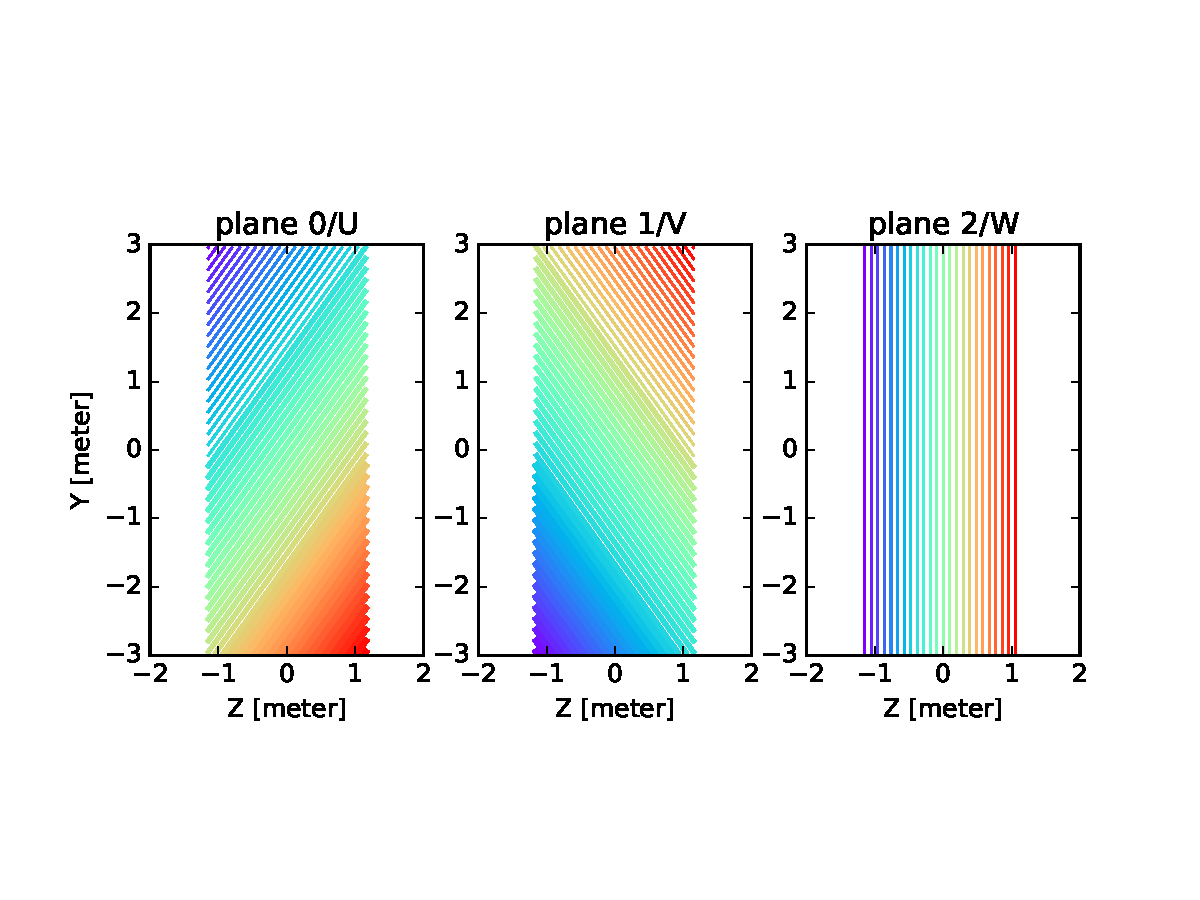
\includegraphics[width=\textwidth,clip,trim=0 3cm 0 3cm]{wires-20.pdf}
  \caption{The wire (segments) for each wire plane on one face of one APA for protoDUNE.  Increasing line width indicates increasing \textbf{segment number} $\in$ (0, 1 or 2).  The color indicates increasing \textbf{wire index} from blue to red.  Only one of every twenty wires are shown. The Y coordinate points opposite of gravity.  The unlabeled X coordinate runs into the page and is counter to the drift direction.  Z follows from the right-hand-rule.  \fixme{Check that U/V are not swapped.}}
  \label{fig:wires}
\end{figure}


\subsection{Wires indices}

Wire indices count wire segments in one plane in the the pitch
direction of the plane.  The count starts from 0 at the smallest (most
negative) $z_w$ (section~\ref{sec:coordsys}).  In
Figure~\ref{fig:wires}, increasing wire index is represented by the
colors transitioning from blue to red.

\subsection{Wire segment index}

The segments that make up a whole conductor are counted starting at
zero from the segment directly attached to a channel input.  The
``collection'' plane wires all have segment index 0.  The conductors
in the wrapped ``induction'' planes may have a maximum segment index
of either 1 or 2.  Increasing segment index is represented by
thickening lines in figure~\ref{fig:wires}.

\subsection{Wire attachment numbers}
\label{sec:wan}

All wires with zero segment index (segment-0 wires) in a given plane
on one face of one APA attach to one of the ten \textit{wire boards}
mounted at the top of the APA frame.  Their \textit{wire attachment
  points} for each plane form an ordered and regular line. 
To match the local numbering convention of the electronics (next
sections) the \textit{wire attachment numbers} count start from 1 and
advance as one goes left-to-right facing the APA.  This means that
they increase with decreasing Z.  Note: the wire attachment numbering
starts counting from 1 to match the convention used by the
electronics. \fixme{The ordering with Z here is from decoding drawings
  and may be swapped!  If so, the numbering directions that follow the
  WAN numbering also need swapping.}

\begin{table}[htp]
  \centering
  \begin{tabular}[h]{ccc}
    \hline
    2/U & 400 & 1 \\
    \hline
    1/V & 400 & 1 \\
    \hline
    0/W & 480 & 1 \\
    \hline
    outer face & $z_c<0$  & $z_c>0$\\
    \hline
    \multicolumn{3}{|c|}{APA frame}\\
    \hline
    inner face & $z_c>0$ & $z_c<0$\\
    \hline
    0/W & 1 & 480 \\
    \hline
    1/V & 1 & 400 \\
    \hline
    2/U & 1 & 400 \\
    \hline
  \end{tabular}
  \caption{Illustration of wire attachement numbers for one APA.  Each wire plane attaches in a line of points at the top of the APA.  These points are counted starting from 1 to match electronics convention and increase as one decreases in the local $z_c$ coordinate.  The numbering is $180^\circ$ rotationally symmetric.}
  \label{tab:wan}
\end{table}

\section{Electronics}

In this note, the electronics consist of all parts carrying signals,
initially analog, from segment-0 wires to, finally digital, the DAQ.

\subsection{ASICs}

Each segment-0 wire attaches to a \textit{wire board}.  There are
ten wire boards per each APA face.  These are numbered in the same
direction as the wire attachment numbers as shown in table~\ref{tab:wireboards}

\begin{table}[htp]
  \label{tab:wireboards}
  \centering
  \begin{tabular}[h]{ccc}
    \hline
     9 & -- & 0 \\
    \hline
    outer face & $z_c<0$  & $z_c>0$\\
    \hline
    \multicolumn{3}{|c|}{APA frame}\\
    \hline
    inner face & $z_c>0$ & $z_c<0$\\
    \hline
    0 & -- & 9 \\
    \hline
  \end{tabular}
  \caption{Wire board numbering.}
\end{table}

Each wire board has attached input wires from all four wire planes
(including grid plane) and locally numbered as shown in
table~\ref{tab:wireboard} matching reference~\cite{docdb2060-v3-adaptor-board-0}.

\begin{table}[htp]
  \label{tab:wireboard}
  \centering
  \begin{tabular}[h]{ccc}
    plane & label & numbering \\
    3 & G & 1 -- 48 \\
    2 & W & 1 -- 48 \\
    1 & V & 1 -- 40 \\
    0 & U & 1 -- 40 \\
  \end{tabular}
  \caption{Local wire board wire attachment numbering.  Numbers
    increase in decreasing $z_c$.  Their numbers go in the same direction as
    wire attachment numbers.}
\end{table}

\noindent Each wire board has associated a front-end motherboard
(FEMB) with eight FEE amplifier and ADC ASIC pairs numbered 1-8.  Each
pair of ASICs has 16 channels numbered 0-15.  The connection from local
wire board attachment number to ASIC number and its local ASIC channel
numbers are nontrivial.  They are exhaustively given in
reference~\cite{wirechmap} and concisely reproduced in a matrix form
in table~\ref{tab:wirechmap}.

The associations represented in this matrix repeat ten times as one
goes down the top of one face of an APA.  This per-face pattern
repeats on the opposite face, obeying a $180^\circ$ rotational
symmetry.

\begin{table}[htp]
  \label{tab:wirechmap}
  \centering
% Note: this table can be generated using chmap.py.

\begin{tabular}{r|rrrrrrrr}
\hline
ASIC:&1&2&3&4&5&6&7&8\\
\hline
ch00 & \textcolor{red}{u19} & \textcolor{red}{u09} & \textcolor{black}{w14} & \textcolor{black}{w02} & \textcolor{red}{u29} & \textcolor{red}{u39} & \textcolor{black}{w26} & \textcolor{black}{w38}\\
ch01 & \textcolor{red}{u17} & \textcolor{red}{u07} & \textcolor{black}{w16} & \textcolor{black}{w04} & \textcolor{red}{u27} & \textcolor{red}{u37} & \textcolor{black}{w28} & \textcolor{black}{w40}\\
ch02 & \textcolor{red}{u15} & \textcolor{red}{u05} & \textcolor{black}{w18} & \textcolor{black}{w06} & \textcolor{red}{u25} & \textcolor{red}{u35} & \textcolor{black}{w30} & \textcolor{black}{w42}\\
ch03 & \textcolor{red}{u13} & \textcolor{red}{u03} & \textcolor{black}{w20} & \textcolor{black}{w08} & \textcolor{red}{u23} & \textcolor{red}{u33} & \textcolor{black}{w32} & \textcolor{black}{w44}\\
ch04 & \textcolor{red}{u11} & \textcolor{red}{u01} & \textcolor{black}{w22} & \textcolor{black}{w10} & \textcolor{red}{u21} & \textcolor{red}{u31} & \textcolor{black}{w34} & \textcolor{black}{w46}\\
ch05 & \textcolor{blue}{v19} & \textcolor{blue}{v09} & \textcolor{black}{w24} & \textcolor{black}{w12} & \textcolor{blue}{v29} & \textcolor{blue}{v39} & \textcolor{black}{w36} & \textcolor{black}{w48}\\
ch06 & \textcolor{blue}{v17} & \textcolor{blue}{v07} & \textcolor{blue}{v12} & \textcolor{blue}{v02} & \textcolor{blue}{v27} & \textcolor{blue}{v37} & \textcolor{blue}{v22} & \textcolor{blue}{v32}\\
ch07 & \textcolor{blue}{v15} & \textcolor{blue}{v05} & \textcolor{blue}{v14} & \textcolor{blue}{v04} & \textcolor{blue}{v25} & \textcolor{blue}{v35} & \textcolor{blue}{v24} & \textcolor{blue}{v34}\\
ch08 & \textcolor{blue}{v13} & \textcolor{blue}{v03} & \textcolor{blue}{v16} & \textcolor{blue}{v06} & \textcolor{blue}{v23} & \textcolor{blue}{v33} & \textcolor{blue}{v26} & \textcolor{blue}{v36}\\
ch09 & \textcolor{blue}{v11} & \textcolor{blue}{v01} & \textcolor{blue}{v18} & \textcolor{blue}{v08} & \textcolor{blue}{v21} & \textcolor{blue}{v31} & \textcolor{blue}{v28} & \textcolor{blue}{v38}\\
ch10 & \textcolor{black}{w23} & \textcolor{black}{w11} & \textcolor{blue}{v20} & \textcolor{blue}{v10} & \textcolor{black}{w35} & \textcolor{black}{w47} & \textcolor{blue}{v30} & \textcolor{blue}{v40}\\
ch11 & \textcolor{black}{w21} & \textcolor{black}{w09} & \textcolor{red}{u12} & \textcolor{red}{u02} & \textcolor{black}{w33} & \textcolor{black}{w45} & \textcolor{red}{u22} & \textcolor{red}{u32}\\
ch12 & \textcolor{black}{w19} & \textcolor{black}{w07} & \textcolor{red}{u14} & \textcolor{red}{u04} & \textcolor{black}{w31} & \textcolor{black}{w43} & \textcolor{red}{u24} & \textcolor{red}{u34}\\
ch13 & \textcolor{black}{w17} & \textcolor{black}{w05} & \textcolor{red}{u16} & \textcolor{red}{u06} & \textcolor{black}{w29} & \textcolor{black}{w41} & \textcolor{red}{u26} & \textcolor{red}{u36}\\
ch14 & \textcolor{black}{w15} & \textcolor{black}{w03} & \textcolor{red}{u18} & \textcolor{red}{u08} & \textcolor{black}{w27} & \textcolor{black}{w39} & \textcolor{red}{u28} & \textcolor{red}{u38}\\
ch15 & \textcolor{black}{w13} & \textcolor{black}{w01} & \textcolor{red}{u20} & \textcolor{red}{u10} & \textcolor{black}{w25} & \textcolor{black}{w37} & \textcolor{red}{u30} & \textcolor{red}{u40}\\
\hline
\end{tabular}


  \caption{The per-FEMB connections between ASIC number (columns), ASIC channel (rows) and the local numbering for wires feeding into the FEMB.  Wires are identified by a local, per-plane count.  Counts are \textcolor{red}{1-40 for U plane and marked in red}, \textcolor{blue}{1-40 for V plane and marked in blue} and \textbf{1-48 for W plane and marked in black}.  As this is for one FEMB, this pattern is applied sequentially 10 times down the top of the APA frame for each APA face.}
\end{table}

\subsection{FEMBs}
\label{sec:fembs}

\fixme{Is there already an APA-local or APA-face-local FEMB numbering?
  If not, what follows is my proposal.}  As partly described in
section~\ref{sec:wan}, there are ten FEMBs per APA face.  To preserve
the same numbering direction as used to label their input wires, the
FEMBs on one APA face are numbered 1-10 from left-to-right as one
looks at a given APA face.  This numbering is 180$^\circ$ symmetric to
the other side.  Or in other words, peering over the top of the APA
one would number the ``other'' side's FEMBs as 10-1 going
left-to-right.  \fixme{Add drawing.}

\subsection{Cold FPGA}

The cold FPGA servicing the eight ADCs on one FEMB multiplexes their
128 channels to four serial output lines which connect (along with
others) to one WIB through a single \textit{cable bundle}.

\fixme{I assume the FPGA adds a local ADC number to the data stream following table~\ref{tab:wirechmap}.  Is it correct?}

\fixme{What is the connectivity graph between ADCs to serial lines?  Are ADCs indeed kept atomic here?}

\fixme{How are the serial lines numbered at the FPGA and at the WIB?}

\fixme{Are the serial lines material to addressing the data?  Ie, if two were swapped at either end, would it make any difference to the final data addressing?}


\subsection{Warm Interface Boards}


The five Warm Interface Boards (WIB) connect to 20 FEMBs on each APA.
Each WIB has a unique IP address derived from crate and slot addresses
for slow-control.  The four serial lines from one cold FPGA are input
to a WIB.  The WIB multiplexes these into one output fiber.  In total,
there are four output fibers, one for each cold FPGA input.  It is
assume that the WIB stamps the outgoing data with numbers for:

\begin{itemize}
\item \textbf{WIB Crate \#} (which corresponds to APA)
\item \textbf{WIB \# in crate} (1-5)
\item \textbf{WIB connector \#} (1-4, corresponding to output fiber number)
\end{itemize}

I can find no FEMB-WIB connectivity graph.  What is give here are two
proposals which are good from the point of view of developing and
viewing online monitoring plots which will use these raw data numbers
and in keeping the mapping from these numbers to offline numbers
simple and regular.  

\textbf{Proposal 1} for the FEMB -- WIB connection is slightly
preferred and is shown in table~\ref{tab:femb-wib-1}.  It groups FEMBs
into \textbf{WIB--major} order, striping neighboring FEMBs across the
same connector on different WIBs.  This means half of one face of one
APA is grouped on one WIB connector number.

\begin{table}[htp]
  \label{tab:femb-wib-1}
  \centering
  \begin{tabular}[h]{|c|c|c|c|c|c|c|c|c|c|}
    \hline
    \multicolumn{10}{|c|}{Cryostat wall} \\
    \hline
    WIB 5 & WIB 4 & WIB 3 & WIB 2 & WIB 1 & WIB 5 & WIB 4 & WIB 3 & WIB 2 & WIB 1 \\
    \multicolumn{5}{|c|}{WIB connector 4} & \multicolumn{5}{c|}{WIB connector 3} \\
    \hline
    \multicolumn{10}{|c|}{APA Frame} \\
    \hline
    \multicolumn{5}{|c|}{WIB connector 1} & \multicolumn{5}{c|}{WIB connector 2} \\
    WIB 1 & WIB 2 & WIB 3 & WIB 4 & WIB 5 & WIB 1 & WIB 2 & WIB 3 & WIB 4 & WIB 5\\
    \hline
    \multicolumn{10}{|c|}{TPC} \\
    \hline
  \end{tabular}
  \caption{FEMB-WIB connectivity proposal \#1.  The table shows mapping from the $2\times10$ physical FEMB location on the top of the APA to WIB addresses following a $1\times5\times4$ layout.}
\end{table}



\textbf{Proposal 2} for the FEMB -- WIB connection is less preferred
but is the only other possible layout which provides the high degree
of hierarchical symmetry.  If looking at the WIB flange, the two
proposals are similar to a matrix transpose of each other.  This
proposal uses \textbf{WIB-connector-major} ordering of a group of
FEMBs, striping a $2\times2$ block of FEMBs across the connectors of
one FEMB.  This proposal is illustrated  in table~\ref{tab:femb-wib-2}.


\begin{table}[htp]
  \label{tab:femb-wib-2}
  \centering
  \begin{tabular}[h]{|c|c|c|c|c|c|c|c|c|c|}
    \hline
    \multicolumn{10}{|c|}{Cryostat wall} \\
    \hline
    WC 4 & WC 3 & WC 4 & WC 3 & WC 4 & WC 3 & WC 4 & WC 3 & WC 4 & WC 3 \\
    \multicolumn{2}{|c|}{WIB 1} & \multicolumn{2}{c|}{WIB 2} & \multicolumn{2}{c|}{WIB 3} & \multicolumn{2}{c|}{WIB 4} & \multicolumn{2}{c|}{WIB 5} \\
    \hline
    \multicolumn{10}{|c|}{APA Frame} \\
    \hline
    \multicolumn{2}{|c|}{WIB 1} & \multicolumn{2}{c|}{WIB 2} & \multicolumn{2}{c|}{WIB 3} & \multicolumn{2}{c|}{WIB 4} & \multicolumn{2}{c|}{WIB 5} \\
    WC 1 & WC 2 & WC 1 & WC 2 & WC 1 & WC 2 & WC 1 & WC 2 & WC 1 & WC 2 \\
    \hline
    \multicolumn{10}{|c|}{TPC} \\
    \hline
  \end{tabular}
  \caption{FEMB-WIB connectivity proposal \#2.  The table shows mapping from the $2\times10$ physical FEMB location on the top of the APA to WIB addresses following a $2\times2\times5$ layout.  Here ``WC'' stands for ``WIB connector''.}

\end{table}

\fixme{Where and in what manner does data from one FEMB get numbered?  Is it indeed the WIB that stamps one FEMB's data with an FEMB number?}


\section{DAQ}

For the purpose of this note, the DAQ includes the dedicated readout
hardware (RCE and FELIX) and the distributed artDAQ application.

\subsection{RCE and FELIX}

Five of the APAs will have their WIBs read out by RCE and one by FELIX
devices.  The DAQ group has committed to providing unpacking code for
the data from both devices to make the resulting data follow identical
schema independent from whether that data came through RCE or FELIX.

\fixme{What is the connectivity between the 2 RCEs/APA and the 5 WIBs/APA?}

\fixme{Where and in what manner does an APA get numbered?}

\fixme{What connectivity graph matters for FELIX?}

\section{Global Numbering}

Each numbering given above is local to a unique part of the detector.
As such a hierarchy of numbers is required to uniquely identify a
specific part.  With some redundancy, the list of quantities that may
be specified are summarized from the above sections as:

\begin{itemize}
\item $G_{tpc}$ global TPC number (central: 1-6 and edge: 7-12)
\item $G_{apa}$ global APA number (1-6)
\item $L_{face}$ local APA face (0,1)
\item $L_{wib}$ local WIB number (5, numbered like ??)
\item $L_{femb}$ local FEMB number on one face (1-10)
\item $L_{asic}$ local ASIC (pair, either FEE amplifier or ADC) on FEMB (1-8)
\item $L_{ch}$ local channel on ASIC (0-15)
\item $L_{plane}$ local wire plane in face (0/U, 1/V, 2/W).
\item $L_{seg}$ local wire segment index in conductor (W always 0, U/V $\in$ 0,1,2)
\item $L_{pitch}$ local wire pitch index in plane
\item $L_{wan}$ local wire attachment number on face of APA (U/V:1-400, W:1-480)
\end{itemize}

The connections between these numbers are very ``shuffled'' due to
wire wrapping, ASIC-wire channel connections, FEMB-WIB cable
connections, multiple APAs and the dichotomy of ``inner'' and
``outer'' faces.  There are also multiple levels in this hierarchy
which are interesting to access.  As such there is clearly no ideal
transformation to produce some a single global number suitable for all
parts and all contexts.  Any choice for such a global number will be
unsuitable for some subset of use cases.  This note makes no proposal
for one single convention.

Rather, it suggests one possible convention and as a family of global
numbering conventions which traverse the hiearchy.  Going in top-down
order, one obvious flattening presents itself:

\[  G_{face} = 1 + (G_{apa}-1) + 2\times L_{face} = G_{tpc} \in (1-12) \]
  
\[  G_{femb} = L_{femb} + 10\times (G_{face}-1) \in (1,120) \]

\[  G_{asic} = L_{asic} + 8\times (G_{femb}-1) \in (1,960) \]

\[ G_{ch} = L_{ch} + 16\times (G_{asic}-1) \in (0,15369) \]

Plots produced in terms of any of the above levels of granularity can
illustrate any effects which are localized to the corresponding
electronics unit.  However, effects that are localized in terms of
wires will not show well in such electronics units due to the
shuffling given in table~\ref{tab:wirechmap}.  A global wire
attachment number $L_{wan}$ can be constructed similarly to $G_{ch}$.

\fixme{Type out $L_{wan}$.}

\section{Concluding remarks}

This note describes the numbers used by the makers of those detector
parts of the single-phase protoDUNE experiment related to TPCs.  Such
numbers are necessarily \textit{local} (as defined in this note).  In
addition to these, some intermediate and global numbering conventions
are proposed.

What remains are two substantial tasks.  \fixme{A third substantial
  task is fixing all the fixmes in this draft.}  First, a system is
needed which represents these as-designed numbers in machine readable
form.  Starting from this ideal basis, methods to identify and record
deviations from the ideal are needed.  Such deviations will occur, be
discovered and possibly be rectified all on differing time scales and
the system must accommodate that.  From the basis and the recorded
deviations it must be possible to produce and reproduce the full local
number hierarchy and at least the more popular flattened
transformations for our state of knowledge at any given time.

The second substantial effort is to develop and apply transformations
of these sets of numbers to sets which are suitable for a given
problem domain or context.  A main example of this is to transform
addresses in the raw data to alternatives which follow conventions and
assumptions that have become baked into LArSoft code.  Other analyses,
monitoring, data processing, engineering will likely also require
their own unique transformations.


\end{document}

%%% Local Variables:
%%% mode: latex
%%% TeX-master: t
%%% End:
